\documentclass[a4j,11pt,dvipdfmx]{jsarticle}
\usepackage{float}
\usepackage{array}
\usepackage{titlesec}
\usepackage[dvipdfmx]{graphicx}
\usepackage{graphicx}
\usepackage{url}

\titleformat*{\section}{\bfseries}
\titleformat*{\subsection}{\bfseries}

\makeatletter
  \renewcommand{\section}{%
    \@startsection{section}{1}{\z@}%
    {0.4\Cvs}{0.1\Cvs}%
    {\normalfont\headfont\raggedright}}
\makeatother

\makeatletter
  % sectionの下マージンを小さく
  \renewcommand{\subsection}{%
    \@startsection{subsection}{1}{\z@}%
    {0.1\Cvs}{0.1\Cvs}%
    {\normalfont\headfont\raggedright}}
\makeatother

\renewcommand{\thesubsection}{\thesection-\arabic{subsection}.}


%---------------------------------------------------
% ページの設定
%---------------------------------------------------
\setlength{\textwidth}{160truemm}
\setlength{\textheight}{250truemm}
\setlength{\topmargin}{-4.5truemm}
\setlength{\oddsidemargin}{0.5truemm}
\pagestyle{empty}
\setlength{\headheight}{0truemm}
\setlength{\parindent}{1zw}
\newcolumntype{b}{!{\vrule width 1pt}}
\newcommand{\bhline}{\noalign{\hrule height 1pt}}   


\begin{document}
提出日: \today
\begin{center}
\huge{進捗報告}\vskip20pt
\large{24G1051 久峩丈}
\end{center}
\begin{flushright}
\end{flushright}
% \begin{table}[H]
%   \centering
%   \begin{tabular}{bp{15.5truecm}b}
%   \bhline
%   \large{\bf{}}
%   \\ \bhline
% \end{tabular}
% \end{table}


%%%%%%%%%%%%%%%%%%%%%%%%%%%%%%%%%%%%%%%%%%%%%%%%%
%%%%%%%%%%%%%%%%%%%%%%%%%%%%%%%%%%%%%%%%%%%%%%%%%
%%%%%%%%%%%%%%%%%%%%%%%%%%%%%%%%%%%%%%%%%%%%%%%%%
\section{第7週進捗状況}

\begin{itemize}
    \item テキスト入力→特定の周波数の音を出力するプログラムの完成
    \begin{itemize}
        \item チームで共有された4進数変換コードを利用して2桁ずつ取得しそれに対応する周波数を出力するコードの記述
    \end{itemize}
    \item 音を出力する回路,回路図の完成
\end{itemize}
% 音通信(送信側)の回路図を図\ref{fig:circuit}に示す.

% \begin{figure}[h]
%     \centering
%     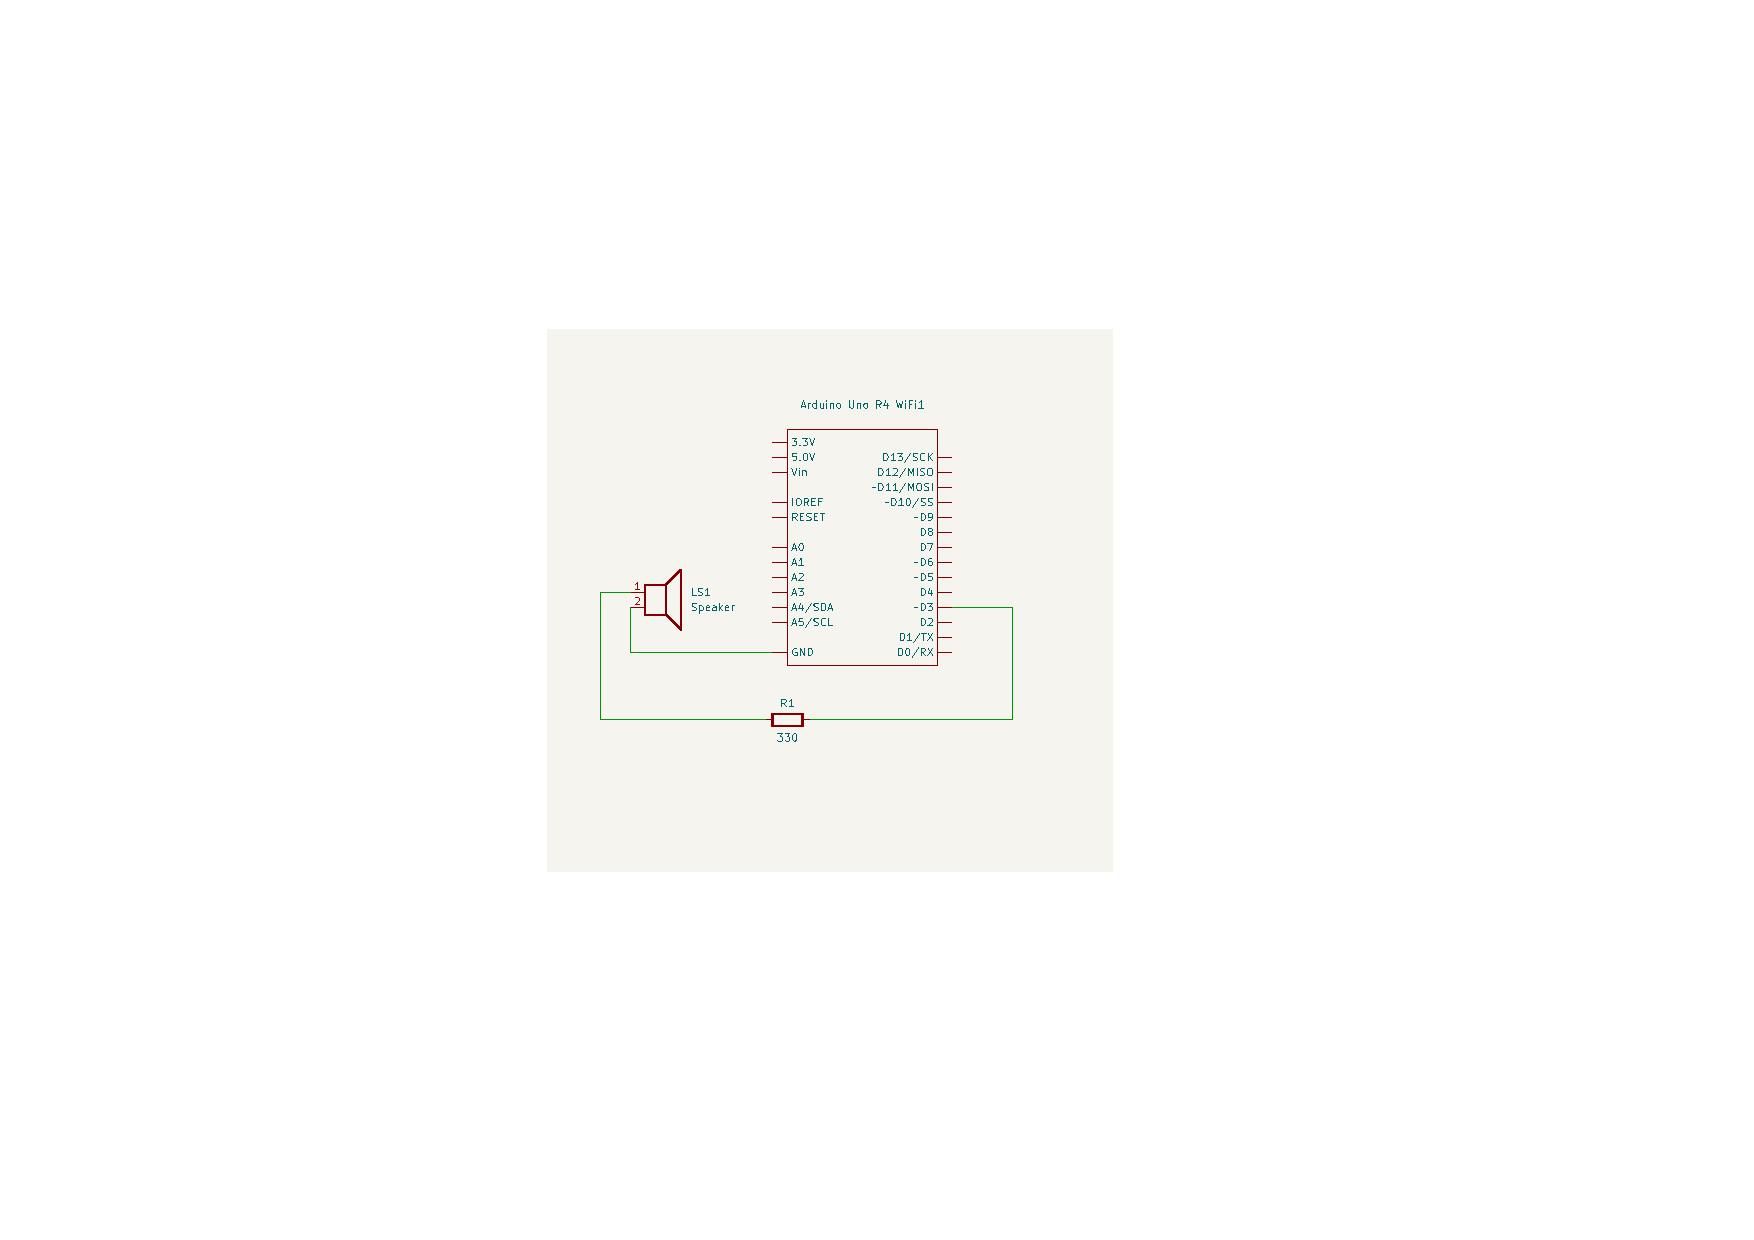
\includegraphics[width=60mm]{/Users/kg/Desktop/university/3S/hack/img/cuircit/sound_tx_cuircit.pdf}
%     \caption{音通信(送信側)の回路図}
%     \label{fig:circuit}
% \end{figure}



\subsection{前回の課題の解決}
スピーカー特性マイク特性ともに機材のデータシートから16種類の周波数の出力,入力に問題ないことを確認した.
また,出力する周波数は450 Hz$\sim$3850 Hzの250 Hz間隔の17種類で,開始と終了の合図用の周波数は450 Hzに設定する.
音送信の回路の電力についてはmacの電源で十分であることを確認した.
光受信の回路(照度センサと抵抗)を含めても十分であると思われる.

%------------------------------------------------%
\section{課題点}
現状の問題としては以下のことが挙げられる.
\begin{itemize}
    \item スピーカーの指向性の考慮
    \begin{itemize}
        \item スピーカーをスタンドなどに設置してマイクに向ける
        \item スピーカーに円錐形の覆いを付ける
    \end{itemize}
    \item 抵抗が$330\Omega$では10mの通信ができないかもしれないため,必要に応じて別途$330\Omega$以下の抵抗器を購入する
    \begin{itemize}
        \item 距離が離れた際スピーカーからの音は小さくなりノイズの影響が相対的に強くなるため,これに耐えうるノイズ除去の実装
    \end{itemize}
\end{itemize}


\section{連携する点}
特定の周波数の音を出力するプログラムと光受信プログラムの結合.
現状ではテキスト入力による出力のみの実装であるため,LED光を受信→4進数数列に変換→対応する音の出力の流れの完成を目指す.

%%%%%%%%%%%%%%%%%%%%%%%%%%%%%%%%%%%%%%%%%%%%%%%%%
%%%%%%%%%%%%%%%%%%%%%%%%%%%%%%%%%%%%%%%%%%%%%%%%%

\end{document}
